\section{Stromrichter und Motor}
Die Funktionsweise des Peugeots unterscheidet sich stark von der des \textsc{Detroits}. Aus diesem Grund soll an dieser Stelle ebenfalls kurz auf den Peugeot eingegangen werden, um aufzuzeigen, welche Lösung bei modernen Elektrofahrzeugen gewählt wird. Die Lösung des Peugeots kann stellvertretend für die meisten anderen modernen Elektrofahrzeuge präsentiert werden, da alle auf einem ähnlichem Prinzip beruhen. Selbst moderne Eisenbahnfahrzeuge sind ähnlich aufgebaut, jedoch mit einem grossen Unterschied: Die Energie wird nicht als Gleichspannung aus einer Batterie geliefert, sondern kommt (als Gleich- oder Wechselspannung) meist mit höherer Spannung aus einem Fahrdraht.

Im Gegensatz zum \textsc{Detroit}, der eine klassische Gleichstrommaschine verwendet, ist der Peugeot mit einer Drehfeldmaschine ausgerüstet. Diese Motoren besitzen gegenüber der Gleichstrommaschine mehrere Vorteile. Durch den Wegfall der Bürsten (Asynchronmaschine und permanenterregte Synchronmaschine) beziehungsweise durch deren deutlich geringerer Belastung (Synchronmaschine) kann die Wartung reduziert werden. Auch sind, insbesondere bei Synchronmaschinen, bei gleicher Leistung kompaktere Motoren im Vergleich zur Gleichstrommaschine möglich.

Im klassischen Fall werden Synchronmaschinen nicht als Motor, sondern in Kraftwerken als Generator verwendet. Der Asynchronmotor hingegen ist die Standardmaschine am dreiphasigen Netz (Drehstrom), wie es in der Schweiz vorhanden ist. Durch das Aufkommen von Stromrichtern, die es einfach ermöglichen Wechselspannung in Gleichspannung und umgekehrt umzuwandeln und folglich auch Wechselspannung einer Frequenz in Wechselspannung einer anderen Frequenz (über den Zwischenschritt der Gleichspannung) wurde beiden Maschinentypen ein weiteres Anwendungsgebiet eröffnet. Dies ist bei drehzahlvariablen Antrieben.

Ein solcher Stromrichter ist auch im Peugeot eingebaut. Da aus der Batterie bereits Gleichspannung bezogen wird, entfällt im Vergleich zum Frequenzumrichter die erste Stufe der Gleichrichtung. Ein Beispiel für einen Stromrichter, wie er im Peugeot verwendet wird, ist in Abbildung \ref{fig:Bruecke} gegeben.

\begin{figure}[h!]
	\centering
		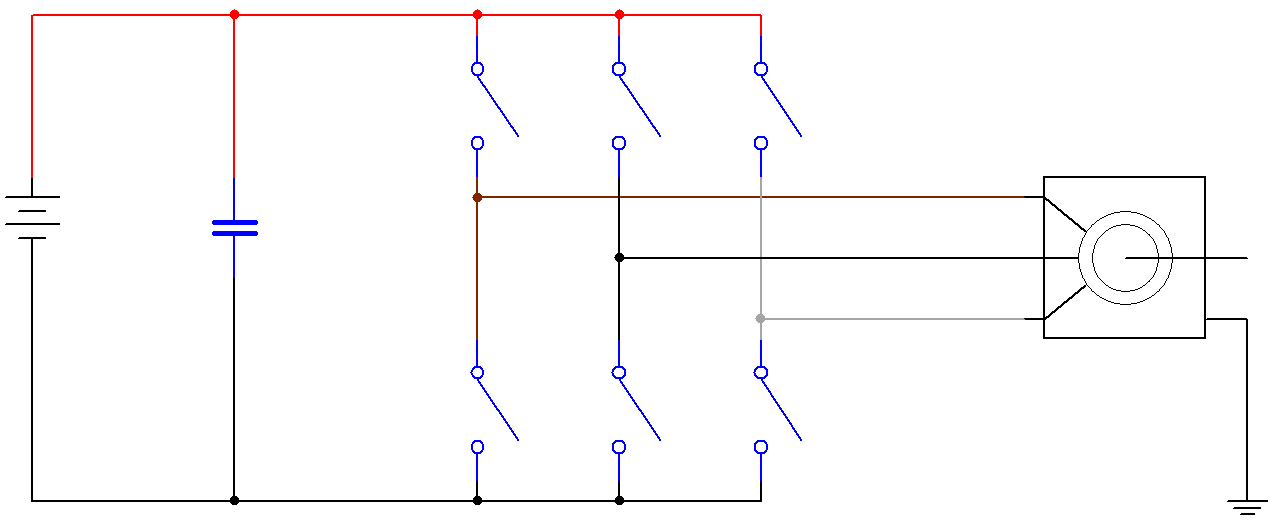
\includegraphics[width=0.80\textwidth]{images/Bruecke.PNG}
	\caption{Aufbau einer dreiphasigen Brücke}
	\label{fig:Bruecke}
\end{figure}

\newpage

Die sechs Transistoren dienen dabei als Schalter, können also nur ein- oder ausgeschaltet sein. In jedem senkrechten Pfad ist nur jeweils ein Schalter eingeschaltet, da es ansonsten zu einem Kurzschluss kommen würde. Durch die beiden Schalter kann der jeweilige Abgang entweder auf den positiven oder den negativen Anschluss der Batterie gelegt werden. Wird dies genügend schnell durchgeführt und der Abgang anschliessend gemittelt (dies kann durch die Induktivität des Motors angenommen werden), so kann dabei jede beliebige Spannungsform erreicht werden. Ein einfaches Beispiel für das Resultat dieser Schaltung kann die Nachbildung des Drehstromnetzes, wie wir es vom schweizerischen Landesnetz kennen, sein. Mit diesem sogenannten Drehfeld kann der Motor in Bewegung gesetzt werden. In Abbildung \ref{fig:Phasenspannungen} ist ein sogenannter Dreiphasendrehstrom dargestellt. Die Spannungen der einzelnen Phasen sind dabei um $120^\circ$ phasenverschobene Sinusfunktionen.

\begin{figure}[h!]
	\centering
		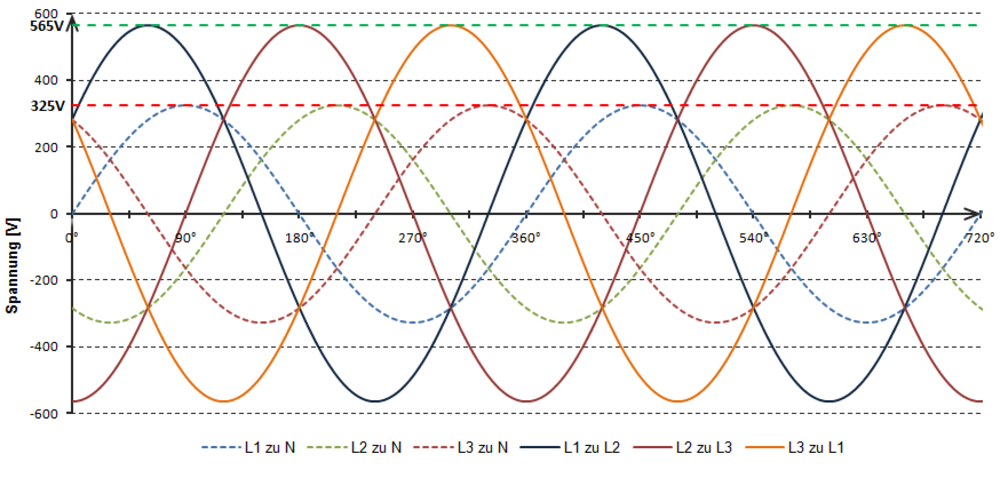
\includegraphics[width=1.00\textwidth]{images/Phasenspannungen.PNG}
	\caption{Phasenspannungen und verkettete Spannungen am Beispiel des $400$ VAC/$50$ Hz-Drehstromnetzes \cite{phasen}}
	\label{fig:Phasenspannungen}
\end{figure}

Drehfeldmaschinen bieten gegenüber Gleichstrommaschinen einen weiteren Vorteil: Wird eine Ausgangsfrequenz des Stromrichters eingestellt, so dreht sich die Maschine ebenfalls mit dieser Frequenz (Synchronmaschine) beziehungsweise aufgrund des Schlupfes um einige Prozent langsamer (Asynchronmaschine). Versucht nun der Motor, durch aufgenommene Leistung an der Welle, schneller zu drehen als das Feld, so wird er automatisch zum Generator und bremst dabei das Fahrzeug. Dabei muss dieser Vorgang für beide Motorentypen unterschieden werden.

Bei \textbf{Asynchronmaschinen} dreht sich funktionsbedingt der Rotor immer etwas langsamer als das Feld, diese Differenz wird auch Schlupf genannt. Ist die Maschine im Nennbetrieb, so kann die Vereinfachung getroffen werden, dass das abgegebene Moment proportional zum Schlupf ist. Folglich ist also bei gleicher Drehzahl kein Moment mehr an der Welle abgreifbar. Wird die mechanische Drehzahl grösser als die sogenannte Synchronfrequenz (kein Schlupf), so wird der Schlupf negativ und folglich auch das Moment an der Welle. Die Maschine nimmt also mechanische Leistung auf und gibt diese als elektrische Leistung ab.

\textbf{Synchronmaschinen} funktionieren anders als Asynchronmaschinen. Der Name kommt daher, dass sie stets mit der selben Drehzahl wie das Feld drehen. Ähnlich wie beim Schlupf der Asynchronmaschine gibt es auch hier eine das Moment beeinflussende Grösse. Im Motorbetrieb läuft der Rotor dem Statorfeld hinterher. Der Winkelversatz ist dabei verantwortlich für das abgegebene Moment (beziehungsweise umgekehrt, das Moment bestimmt den Winkelversatz). Wird dieser Winkelversatz null, der Stator läuft also exakt mit dem Rotorfeld mit, so ist auch das abgegebene Moment null. Wenn der Rotor dem Drehfeld voraus eilt, so ändert sich auch hier die Richtung des elektrischen Energieflusses.

Die so erzeugte Energie ist in beiden Fällen eine dreiphasige Wechselspannung. Mit Hilfe des Stromrichters wird dadurch wieder eine konstante Gleichspannung erzeugt, mit welcher beim Bremsen die Batterie aufgeladen werden kann (dies wird auch als Rekuperation bezeichnet). Dadurch kann zur Bremsung des Fahrzeuges einfach die Frequenz unterhalb der Motorendrehzahl gehalten werden (Asynchronmaschine) beziehungsweise, bildlich gesprochen, $"$kurz gewartet werden$"$, bis der Rotor dem Drehfeld voreilt (Synchronmaschine).

Die hier vorgestellten Vorgänge benötigen ein hohes Mass an Regelung. Zusätzlich zu den Schaltelementen kommt in jedem Stromrichter noch ein Prozessor hinzu, der den gesamten Zustand regelt. Auch sind viele weitere Schaltungsteile nötig, um beispielsweise eine galvanische Trennung, eine Messung der elektrischen Grössen oder die Überwachung der Schaltertemperaturen durchzuführen. Diese sollen jedoch an dieser Stelle nicht weiter behandelt werden. Es sollte nur die grundsätzliche Funktionsweise des Stromrichters erklärt werden.

Auch Gleichstrommaschinen, wie die im \textsc{Detroit} verbaute, können als Generator benutzt werden. Beim \textsc{Detroit} war dies jedoch trotzdem nicht möglich. Für genauere Informationen sei auf das Kapitel \ref{bremse} verwiesen.
%Natürlich kann auch eine Gleichstrommaschine als Generator benutzt werden. Zu diesem Zweck muss die induzierte Spannung (siehe Kapitel \ref{gm}) grösser werden als die Batteriespannung. Da sich dadurch aber auch die Stromrichtung umdreht, wird bei der Reihenschlussmaschine das Erregerfeld ebenfalls gekehrt, was die Nutzung als Generator verhindert. Für die Nutzung als Generator wäre also eine fremderregte Maschine benötigt worden. Dies wäre beim \textsc{Detroit} schaltungstechnisch möglich gewesen, aufgrund der stark variierenden Drehzahlen wäre jedoch ebenfalls ein Stromrichter nötig gewesen, um die Spannung des Generators an die Batteriespannung anzupassen.

Für weitere, ausführlichere Informationen zu Drehfeldmaschinen und die dazugehörigen Stromrichter sei auf die Literatur \cite{elektrischeantriebe} verwiesen.

\newpage